\subsection{The ordinary service fails before the investment loop}

\textbf{No world produces positive ordinary operating surplus.} Across all 384 worlds,
available earned investment funds remain exactly zero in every week. No first or second
capability is acquired, and no succession repays. The four policy results are identical
because every policy retains A. This is an operating-demand/cost failure before a capability
funding event, not a claim that graph execution caused the losses.

\begin{longtable}{@{}llllrrr@{}}
\caption{All 24 primary economic conditions, 16 seeds each. Mean accepted jobs and USD results.
Policies A/B/C/D coincide because no purchase is admitted. I is buyer integration minutes.}\\
\toprule Demand & I & Competitor & Cost & Jobs & Operating & Project\\ \midrule\endfirsthead
\toprule Demand & I & Competitor & Cost & Jobs & Operating & Project\\ \midrule\endhead
low & 0 & strong & low & 0.00 & -448.76 & -573.18 \\
low & 0 & strong & reference & 0.00 & -509.20 & -1011.83 \\
low & 0 & equal & low & 1.00 & -447.18 & -571.60 \\
low & 0 & equal & reference & 0.00 & -509.20 & -1011.83 \\
low & 15 & strong & low & 0.00 & -448.76 & -573.18 \\
low & 15 & strong & reference & 0.00 & -509.20 & -1011.83 \\
low & 15 & equal & low & 0.81 & -445.54 & -569.96 \\
low & 15 & equal & reference & 0.00 & -509.20 & -1011.83 \\
reference & 0 & strong & low & 0.00 & -448.76 & -573.18 \\
reference & 0 & strong & reference & 0.00 & -509.20 & -1011.83 \\
reference & 0 & equal & low & 4.25 & -439.42 & -563.84 \\
reference & 0 & equal & reference & 0.00 & -509.20 & -1011.83 \\
reference & 15 & strong & low & 0.00 & -448.76 & -573.18 \\
reference & 15 & strong & reference & 0.00 & -509.20 & -1011.83 \\
reference & 15 & equal & low & 4.19 & -430.30 & -554.72 \\
reference & 15 & equal & reference & 0.00 & -509.20 & -1011.83 \\
high & 0 & strong & low & 0.00 & -448.76 & -573.18 \\
high & 0 & strong & reference & 0.00 & -509.20 & -1011.83 \\
high & 0 & equal & low & 8.75 & -410.80 & -535.22 \\
high & 0 & equal & reference & 0.00 & -509.20 & -1011.83 \\
high & 15 & strong & low & 0.00 & -448.76 & -573.18 \\
high & 15 & strong & reference & 0.00 & -509.20 & -1011.83 \\
high & 15 & equal & low & 9.75 & -391.55 & -515.97 \\
high & 15 & equal & reference & 0.00 & -509.20 & -1011.83 \\
\bottomrule\end{longtable}

The most favorable cell mean is high arrival, 15-minute buyer integration, equal competition
and low operating cost: 9.75 accepted jobs, \$153.28 simulated collections, \$391.55 operating
loss and \$515.97 modeled project loss. This is a post-run descriptive maximum, not a newly
selected confirmatory condition. Even the best individual world loses \$233.97 operating
and \$358.39 after opening costs: \$408.75 collected versus \$642.72 accrued operating costs
and \$124.42 opening costs. Its cash is \$655.70, unpaid obligations \$14.09 and receivables
\$32.70. Positive cash includes remaining seed and is not profit.

All reference-cost conditions exhaust cash and become insolvent at week 20. Their 19 charged
weeks accrue \$509.20 operating cost, in addition to \$502.63 opening cost, leaving \$11.83
unpaid. All low-cost/strong-competitor conditions collect nothing and lose \$448.76 in recurring
operation, or \$573.18 including opening costs. The model makes refusal, competition and
finite capital consequential rather than replacing missing sales with assumed transfers.

\begin{figure}[htbp]\centering
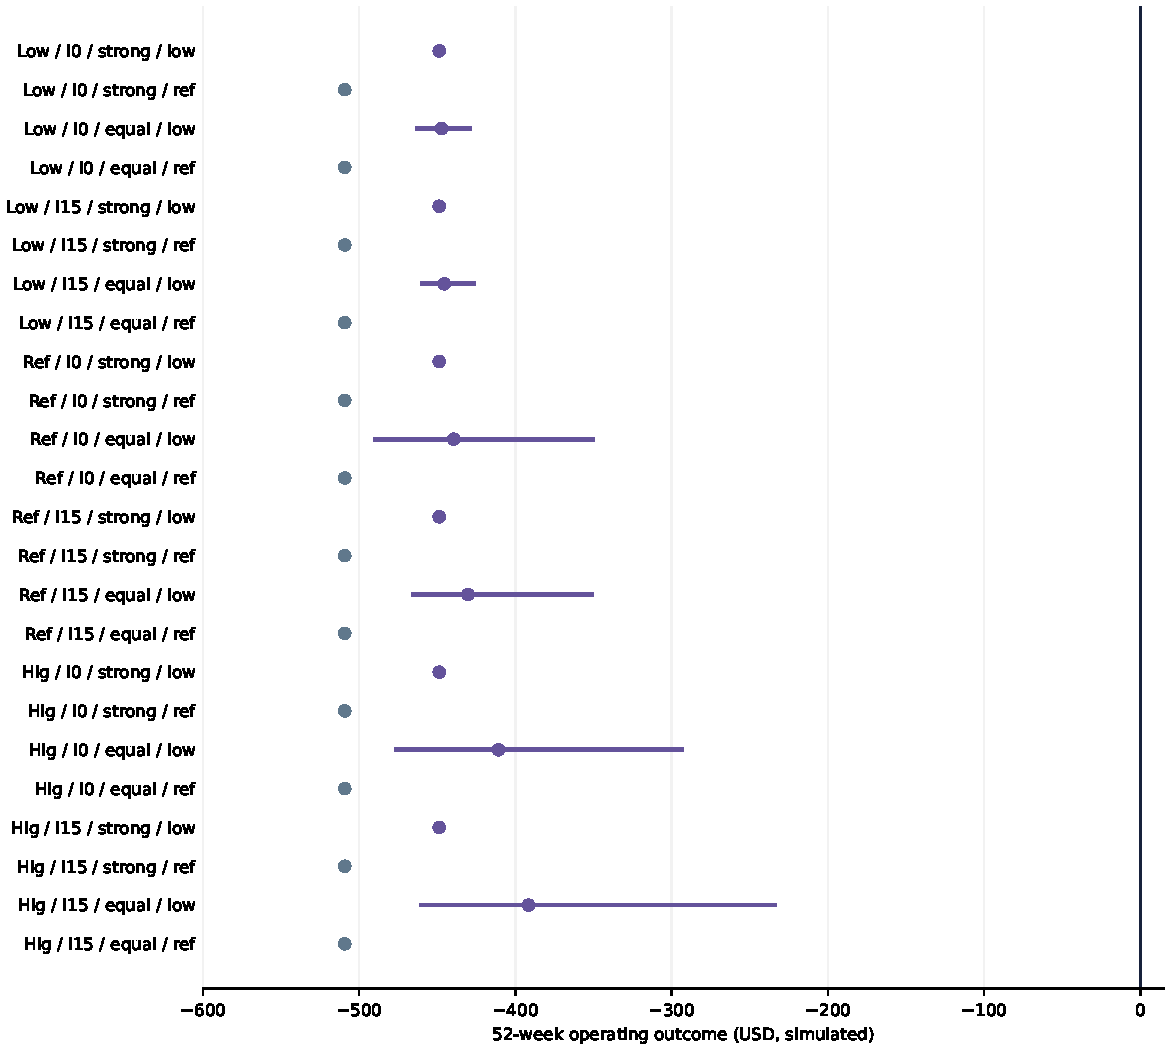
\includegraphics[width=0.95\linewidth]{figures/economic-cells.pdf}
\caption{All predeclared cells. Dots show mean operating outcome across 16 paired seeds; lines
show the full minimum--maximum range, not confidence intervals. Labels show demand, integration,
competition and cost bundle. Every range remains below zero. Reference-cost runs stop after
insolvency; they do not receive an extra seed injection.}
\end{figure}

\subsection{Cheap computation is not a complete service margin}

Including acquisition, failed source handling at the machine level and driver allocation, the
standalone mechanical CPU per accepted question is 1.547, 2.675, 2.891 and 2.744 seconds for
A/B/C/D. At the \emph{assumed} \$1 per CPU-hour, these are far below a cent. The actual billed
machine and inference costs are not known. Residual attention, low conversion and recurring
operation dominate the declared scenarios.

\begin{table}[htbp]\small
\caption{Prospective costing is not realized utilization. All dollar values below are modeled.}
\begin{tabularx}{\linewidth}{@{}Yrr@{}}
\toprule Quantity & Low bundle & Reference bundle\\ \midrule
Expected full prospective cost per collected job at reference utilization & \$15.48 & \$35.10\\
Resulting fixed grid tariff & \$16.35 & \$65.38\\
Historical discovery/setup opening & \$124.42 & \$502.63\\
First capability A to B, complete fixed incremental cost & \$135.77 & \$449.95\\
Second capability B to C, complete fixed incremental cost & \$119.43 & \$363.24\\
Second capability B to D, including graph increment & \$165.53 & \$509.46\\
\bottomrule\end{tabularx}
\end{table}

The best cell's actual modeled utilization produces approximately \$55.88 accrued recurring
cost per accepted job and \$68.64 including its opening allocations (ratios of cell totals).
Those figures differ from the \$15.48 prospective cost because competition and refusal prevent
the assumed reference utilization from being achieved. The grid's reference tariff jumps from
\$35.10 calculated cost to \$65.38, above the maximum modeled willingness to pay. This coarse
pricing choice contributes to refusal; it is a limitation of the tested policy, not empirical
evidence that a continuously priced offering cannot sell. No alternative price campaign was
introduced after observing these outcomes.

Human-only duration remains unmeasured. For example, the assumed 45-minute competent workflow
costs \$49.04 at the wage anchor; a \$16.35 service plus two buyer-review minutes costs \$18.53
before buyer integration. That conditional \$30.51 avoided cost is not observed savings,
enterprise revenue beyond the tariff, or available surplus. Shorter assumed human workflows
can rationally favor self-service. The diagnostic table varies residual attention over 2, 5 and
10 minutes and retains the unknown actual full-cost category.

\subsection{The proposed upgrades also lack a repayment case}

A to B adds 1.128 measured CPU seconds per available accepted question; B to C adds 0.216;
B to D adds 0.068. These signed deltas supply no positive CPU-only saving even at zero incremental
maintenance. The complete candidate investments therefore have no finite CPU-only break-even
reuse or repayment time. Adding the declared maintenance cannot improve that conclusion.
None was financed.

The separate C-to-D graph diagnostic has a 0.147-second observed CPU difference in the favorable
direction, without an added accepted job or identified planning gain. Even if that single-run
difference were stable and credited at \$1 per CPU-hour, the low \$46.10 graph increment would
require over 1.15 million reuses at zero maintenance with the frozen conservative microdollar credit (about 1.159 million under the conservative
cash-rounding diagnostic). Nonzero declared maintenance removes the finite repayment.
This is a sensitivity calculation, not evidence that the measured timing difference generalizes.

At an illustrative 156 execution reuses in 26 weeks, the low-cost A-to-B investment would need
about 0.90 minutes of additional paid attention avoided per reuse to cover its complete cost
and maintenance. No such saving was observed. This is a concrete measurement target for a
future capability test, not a benefit inserted into the present simulation.
